\documentclass[10pt,fleqn]{article} % Default font size and left-justified equations
\usepackage[%
    pdftitle={Modélisation dynamique : cinétique},
    pdfauthor={Xavier Pessoles}]{hyperref}

    
%%%%%%%%%%%%%%%%%%%%%%%%%%%%%%%%%%%%%%%%%
% Original author:
% Mathias Legrand (legrand.mathias@gmail.com) with modifications by:
% Vel (vel@latextemplates.com)
% License:
% CC BY-NC-SA 3.0 (http://creativecommons.org/licenses/by-nc-sa/3.0/)
%%%%%%%%%%%%%%%%%%%%%%%%%%%%%%%%%%%%%%%%%

%----------------------------------------------------------------------------------------
%	VARIOUS REQUIRED PACKAGES AND CONFIGURATIONS
%----------------------------------------------------------------------------------------

%\usepackage[top=2.5cm,bottom=2cm,left=2cm,right=2cm,headsep=40pt,a4paper]{geometry} % Page margins
\usepackage[top=2cm,bottom=3cm,left=2cm,right=2cm,a4paper]{geometry} % Page margins

\usepackage{graphicx} % Required for including pictures

\usepackage{lipsum} % Inserts dummy text

\usepackage{tikz} % Required for drawing custom shapes

\usepackage[francais]{babel} % English language/hyphenation
\frenchbsetup{StandardLists=true} % Pour éviter la collision babel enumitem pour les listes

\usepackage{enumitem} % Customize lists
\setlist{nolistsep} % Reduce spacing between bullet points and numbered lists

\usepackage{booktabs} % Required for nicer horizontal rules in tables

\usepackage{xcolor} % Required for specifying colors by name
%\definecolor{ocre}{RGB}{243,102,25} % Define the orange color used for highlighting throughout the book
 \definecolor{ocre}{RGB}{49,133,156} % Couleur ''bleue''
\definecolor{violetf}{RGB}{112,48,160} % Couleur ''violet''
\usepackage{enumitem}
\usepackage{pifont} % Pour les dinglist
\usepackage{multicol}
\usepackage{array} % Centrage vertical dans les tableaux
\usepackage{schemabloc}

%----------------------------------------------------------------------------------------
%	FONTS
%----------------------------------------------------------------------------------------
\usepackage{bm}
\usepackage{multicol}
\usepackage{siunitx}
\sisetup{output-decimal-marker = {,}}


\usepackage{avant} % Use the Avantgarde font for headings
%\usepackage{times} % Use the Times font for headings
%\usepackage{mathptmx} % Use the Adobe Times Roman as the default text font together with math symbols from the Sym­bol, Chancery and Com­puter Modern fonts
\usepackage[adobe-utopia]{mathdesign}
\usepackage{microtype} % Slightly tweak font spacing for aesthetics
\usepackage[utf8]{inputenc} % Required for including letters with accents
\usepackage[T1]{fontenc} % Use 8-bit encoding that has 256 glyphs

%----------------------------------------------------------------------------------------
%	BIBLIOGRAPHY AND INDEX
%----------------------------------------------------------------------------------------

%\usepackage[style=alphabetic,citestyle=numeric,sorting=nyt,sortcites=true,autopunct=true,babel=hyphen,hyperref=true,abbreviate=false,backref=true,backend=biber]{biblatex}
\usepackage[style=alphabetic,citestyle=numeric,sorting=nyt,sortcites=true,autopunct=true,hyperref=true,abbreviate=false,backref=true,backend=biber]{biblatex}
\addbibresource{bibliography.bib} % BibTeX bibliography file
\defbibheading{bibempty}{}

\usepackage{calc} % For simpler calculation - used for spacing the index letter headings correctly
\usepackage{makeidx} % Required to make an index
\makeindex % Tells LaTeX to create the files required for indexing

%----------------------------------------------------------------------------------------
%	MAIN TABLE OF CONTENTS
%----------------------------------------------------------------------------------------

\usepackage{titletoc} % Required for manipulating the table of contents

\setcounter{tocdepth}{2}     % Dans la table des matieres
\setcounter{secnumdepth}{2}

\contentsmargin{0cm} % Removes the default margin

% Part text styling
\titlecontents{part}[0cm]
{\addvspace{20pt}\centering\large\bfseries}
{}
{}
{}

% Chapter text styling
\titlecontents{chapter}[1.25cm] % Indentation
{\addvspace{12pt}\large\sffamily\bfseries} % Spacing and font options for chapters
{\color{ocre!60}\contentslabel[\Large\thecontentslabel]{1.25cm}\color{ocre}} % Chapter number
{\color{ocre}}  
{\color{ocre!60}\normalsize\;\titlerule*[.5pc]{.}\;\thecontentspage} % Page number

% Section text styling
\titlecontents{section}[1.25cm] % Indentation
{\addvspace{3pt}\sffamily\bfseries} % Spacing and font options for sections
{\color{ocre!60}\contentslabel[\thecontentslabel]{1.25cm} \color{ocre}} % Section number
{\color{ocre}}
{\hfill\color{ocre!60}\thecontentspage} % Page number
[]

% Subsection text styling
\titlecontents{subsection}[1.25cm] % Indentation
{\addvspace{1pt}\sffamily\small} % Spacing and font options for subsections
{\contentslabel[\thecontentslabel]{1.25cm}} % Subsection number
{}
{\ \titlerule*[.5pc]{.}\;\thecontentspage} % Page number
[]


% Subsection text styling
\titlecontents{subsubsection}[1.25cm] % Indentation
{\addvspace{1pt}\sffamily\small} % Spacing and font options for subsections
{\contentslabel[\thecontentslabel]{1.25cm}} % Subsection number
{}
{\ \titlerule*[.5pc]{.}\;\thecontentspage} % Page number
[]

% List of figures
\titlecontents{figure}[0em]
{\addvspace{-5pt}\sffamily}
{\thecontentslabel\hspace*{1em}}
{}
{\ \titlerule*[.5pc]{.}\;\thecontentspage}
[]

% List of tables
\titlecontents{table}[0em]
{\addvspace{-5pt}\sffamily}
{\thecontentslabel\hspace*{1em}}
{}
{\ \titlerule*[.5pc]{.}\;\thecontentspage}
[]

%----------------------------------------------------------------------------------------
%	MINI TABLE OF CONTENTS IN PART HEADS
%----------------------------------------------------------------------------------------

% Chapter text styling
\titlecontents{lchapter}[0em] % Indenting
{\addvspace{15pt}\large\sffamily\bfseries} % Spacing and font options for chapters
{\color{ocre}\contentslabel[\Large\thecontentslabel]{1.25cm}\color{ocre}} % Chapter number
{}  
{\color{ocre}\normalsize\sffamily\bfseries\;\titlerule*[.5pc]{.}\;\thecontentspage} % Page number

% Section text styling
\titlecontents{lsection}[0em] % Indenting
{\sffamily\small} % Spacing and font options for sections
{\contentslabel[\thecontentslabel]{1.25cm}} % Section number
{}
{}

% Subsection text styling
\titlecontents{lsubsection}[.5em] % Indentation
{\normalfont\footnotesize\sffamily} % Font settings
{}
{}
{}

%----------------------------------------------------------------------------------------
%	PAGE HEADERS
%----------------------------------------------------------------------------------------

\usepackage{fancyhdr} % Required for header and footer configuration



\pagestyle{fancy}
 \renewcommand{\headrulewidth}{0pt}
 \fancyhead{}
 
 % ENTETES de page
 \fancyhead[L]{%
 \noindent\begin{minipage}[c]{2.6cm}%
 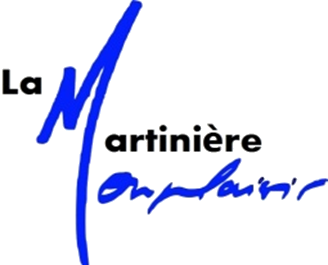
\includegraphics[width=2cm]{logo_lycee.png}%
 \end{minipage}
}

\fancyhead[C]{\rule{8cm}{.5pt}}

 \fancyhead[R]{%
 \noindent\begin{minipage}[c]{3cm}
 \begin{flushright}
 \footnotesize{\textit{\textsf{\xxtete}}}%
 \end{flushright}
 \end{minipage}
}

 \fancyfoot{}
 % PIEDS de page
\fancyfoot[C]{\rule{12cm}{.5pt}}
\renewcommand{\footrulewidth}{0.2pt}
\fancyfoot[C]{\footnotesize{\bfseries \thepage}}
\fancyfoot[L]{ 
\begin{minipage}[c]{.4\linewidth}
\noindent\footnotesize{{\xxauteur}}
\end{minipage}}

\fancyfoot[R]{\footnotesize{\xxpied}
\ifthenelse{\isodd{\value{page}}}{
\begin{tikzpicture}[overlay]
\node[shape=rectangle, 
      rounded corners = .25 cm,
	  draw= ocre,
	  line width=2pt, 
	  fill = ocre!10,
	  minimum width  = 2.5cm,
	  minimum height = 3cm,] at (\xxposongletx,\xxposonglety) {};
\node at (\xxposonglettext,\xxposonglety) {\rotatebox{90}{\textbf{\large\color{ocre}{\xxonglet}}}};
%{};
\end{tikzpicture}}{}
}



%
%
%
% Removes the header from odd empty pages at the end of chapters
\makeatletter
%\renewcommand{\cleardoublepage}{
%\clearpage\ifodd\c@page\else
%\hbox{}
%\vspace*{\fill}
%\thispagestyle{empty}
%\newpage
%\fi}

%\fancypagestyle{plain}{%
%\fancyhf{} % vide l’en-tête et le pied~de~page.
%%\fancyfoot[C]{\bfseries \thepage} % numéro de la page en cours en gras
%% et centré en pied~de~page.
%\fancyfoot[R]{\footnotesize{\xxpied}}
%\fancyfoot[C]{\rule{12cm}{.5pt}}
%\renewcommand{\footrulewidth}{0.2pt}
%\fancyfoot[C]{\footnotesize{\bfseries \thepage}}
%\fancyfoot[L]{ 
%\begin{minipage}[c]{.4\linewidth}
%\noindent\footnotesize{{\xxauteur}}
%\end{minipage}}}

\fancypagestyle{plain}{%
\fancyhf{} % vide l’en-tête et le pied~de~page.
\fancyfoot[C]{\rule{12cm}{.5pt}}
\renewcommand{\footrulewidth}{0.2pt}
\fancyfoot[C]{\footnotesize{\bfseries \thepage}}
\fancyfoot[L]{ 
\begin{minipage}[c]{.4\linewidth}
\noindent\footnotesize{{\xxauteur}}
\end{minipage}}
\fancyfoot[R]{\footnotesize{\xxpied}}
}




%----------------------------------------------------------------------------------------
%	THEOREM STYLES
%----------------------------------------------------------------------------------------

% Conflit avec la police adobe
%\usepackage{amsmath,amsfonts,amssymb,amsthm} % For math equations, theorems, symbols, etc
\usepackage{amsmath,amsthm}

\newcommand{\intoo}[2]{\mathopen{]}#1\,;#2\mathclose{[}}
\newcommand{\ud}{\mathop{\mathrm{{}d}}\mathopen{}}
\newcommand{\intff}[2]{\mathopen{[}#1\,;#2\mathclose{]}}
%\newtheorem{notation}{Notation}[chapter]
\newtheorem{notation}{Notation}[section]

% Boxed/framed environments
\newtheoremstyle{ocrenumbox}% % Theorem style name
{0pt}% Space above
{0pt}% Space below
{\normalfont}% % Body font
{}% Indent amount
{\small\bf\sffamily\color{ocre}}% % Theorem head font
{\;}% Punctuation after theorem head
{0.25em}% Space after theorem head
{\small\sffamily\color{ocre}\thmname{#1}\nobreakspace\thmnumber%{\@ifnotempty{#1}{}\@upn{#2}}% Theorem text (e.g. Theorem 2.1)
\thmnote{\nobreakspace\the\thm@notefont\sffamily\bfseries\color{black}---\nobreakspace#3.}} % Optional theorem note
\renewcommand{\qedsymbol}{$\blacksquare$}% Optional qed square


% Boite pour les corriges
\newtheoremstyle{correctionbox}% % Theorem style name
{0pt}% Space above
{0pt}% Space below
{\normalfont}% % Body font
{}% Indent amount
{\small\bf\sffamily\color{violet}}% % Theorem head font
{\;}% Punctuation after theorem head
{0.25em}% Space after theorem head
{\small\sffamily\color{ocre}\thmname{#1}\nobreakspace\thmnumber%{\@ifnotempty{#1}{}\@upn{#2}}% Theorem text (e.g. Theorem 2.1)
\thmnote{\nobreakspace\the\thm@notefont\sffamily\bfseries\color{black}---\nobreakspace#3.}} % Optional theorem note
\renewcommand{\qedsymbol}{$\blacksquare$}% Optional qed square



\newtheoremstyle{blacknumex}% Theorem style name
{5pt}% Space above
{5pt}% Space below
{\normalfont}% Body font
{} % Indent amount
{\small\bf\sffamily}% Theorem head font
{\;}% Punctuation after theorem head
{0.25em}% Space after theorem head
{\small\sffamily{\tiny\ensuremath{\blacksquare}}\nobreakspace\thmname{#1}\nobreakspace\thmnumber%{\@ifnotempty{#1}{}\@upn{#2}}% Theorem text (e.g. Theorem 2.1)
\thmnote{\nobreakspace\the\thm@notefont\sffamily\bfseries---\nobreakspace#3.}}% Optional theorem note

\newtheoremstyle{blacknumbox} % Theorem style name
{0pt}% Space above
{0pt}% Space below
{\normalfont}% Body font
{}% Indent amount
{\small\bf\sffamily}% Theorem head font
{\;}% Punctuation after theorem head
{0.25em}% Space after theorem head
{\small\sffamily\thmname{#1}\nobreakspace 
\thmnote{\nobreakspace\the\thm@notefont\sffamily\bfseries---\nobreakspace#3.}}% Optional theorem note

% Non-boxed/non-framed environments
\newtheoremstyle{ocrenum}% % Theorem style name
{5pt}% Space above
{5pt}% Space below
{\normalfont}% % Body font
{}% Indent amount
{\small\bf\sffamily\color{ocre}}% % Theorem head font
{\;}% Punctuation after theorem head
{0.25em}% Space after theorem head
{\small\sffamily\color{ocre}\thmname{#1}\nobreakspace%\thmnumber{\@ifnotempty{#1}{}\@upn{#2}}% Theorem text (e.g. Theorem 2.1)
\thmnote{\nobreakspace\the\thm@notefont\sffamily\bfseries\color{black}---\nobreakspace#3.}} % Optional theorem note
\renewcommand{\qedsymbol}{$\blacksquare$}% Optional qed square
\makeatother

% Environnement pour les titres de parties
\newtheoremstyle{partiebox} 
{0pt}% Space above
{0pt}% Space below
{\normalfont}% Body font
{}% Indent amount
{\small\bf\sffamily}% Theorem head font
{\;}% Punctuation after theorem head
{0.25em}% Space after theorem head




% Defines the theorem text style for each type of theorem to one of the three styles above
\newcounter{dummy} 
\numberwithin{dummy}{section}
\theoremstyle{ocrenumbox}
%\newtheorem{theoremeT}[dummy]{Théorème}
\newtheorem{theoremeT}[dummy]{Théorème}
\newtheorem{resultatT}[dummy]{Résultat}
\newtheorem{savoirT}[dummy]{Savoir}
\newtheorem{methodeT}[dummy]{Méthode}
\newtheorem{objectifT}[dummy]{Objectif}
%\newtheorem{problem}{Problem}[chapter]
\newtheorem{problem}{Problem}[section]
%\newtheorem{exerciseT}{Exercise}[chapter]
\newtheorem{exerciseT}{Exercice}[section]

\theoremstyle{blacknumex}
%\newtheorem{exampleT}{Example}[chapter]
\newtheorem{exempleT}{Exemple}[section]
\newtheorem{termT}{Terminal\\}[section]
\newtheorem{pyT}{Python\\}[section]
\newtheorem{sciT}{Scilab\\}[section]
\newtheorem{pseudoT}{Pseudo Code\\}[section]
\newtheorem{sqlT}{SQL\\}[section]

\theoremstyle{blacknumbox}
%\newtheorem{vocabulary}{Vocabulary}[chapter]
\newtheorem{vocabulary}{Vocabulaire}[section]
%\newtheorem{definitionT}{Definition}[section]
\newtheorem{definitionT}{Définition}[section]
\newtheorem{rappelT}{Rappel}[section]
\newtheorem{demoT}{Démonstration}[section]
\newtheorem{corollaryT}[dummy]{Corollaire}
\newtheorem{hypoT}{Hypothèse(s)}

\theoremstyle{ocrenum}
\newtheorem{proposition}[dummy]{Proposition}

\theoremstyle{partiebox}
\newtheorem{titrepartieT}[]{}
\newtheorem{titrechapitreT}[]{}

\theoremstyle{correctionbox}
\newtheorem{correctionT}[dummy]{\color{violet}{Correction}}

%----------------------------------------------------------------------------------------
%	DEFINITION OF COLORED BOXES
%----------------------------------------------------------------------------------------

\RequirePackage[framemethod=tikz]{mdframed} % Required for creating the theorem, definition, exercise and corollary boxes

% Theorem box
\newmdenv[skipabove=7pt,
skipbelow=7pt,
backgroundcolor=ocre!10,
linecolor=ocre,
innerleftmargin=5pt,
innerrightmargin=5pt,
innertopmargin=5pt,
leftmargin=0cm,
rightmargin=0cm,
innerbottommargin=5pt]{tBox}


% Correction
\newmdenv[skipabove=7pt,
skipbelow=7pt,
backgroundcolor=violet!10,
linecolor=violet,
innerleftmargin=5pt,
innerrightmargin=5pt,
innertopmargin=5pt,
leftmargin=0cm,
rightmargin=0cm,
innerbottommargin=5pt]{coBox}


% Exercise box	  
\newmdenv[skipabove=7pt,
skipbelow=7pt,
rightline=false,
leftline=true,
topline=false,
bottomline=false,
backgroundcolor=ocre!10,
linecolor=ocre,
innerleftmargin=5pt,
innerrightmargin=5pt,
innertopmargin=5pt,
innerbottommargin=5pt,
leftmargin=0cm,
rightmargin=0cm,
linewidth=4pt]{eBox}	

% Definition box
\newmdenv[skipabove=7pt,
skipbelow=7pt,
rightline=false,
leftline=true,
topline=false,
bottomline=false,
backgroundcolor=ocre!10,
linecolor=ocre,
innerleftmargin=5pt,
innerrightmargin=5pt,
innertopmargin=0pt,
leftmargin=0cm,
rightmargin=0cm,
linewidth=4pt,
innerbottommargin=0pt]{dBox}	

% Demonstration box
\newmdenv[skipabove=7pt,
skipbelow=7pt,
rightline=false,
leftline=true,
topline=false,
bottomline=false,
%backgroundcolor=ocre!10,
linecolor=ocre,
innerleftmargin=5pt,
innerrightmargin=5pt,
innertopmargin=0pt,
leftmargin=0cm,
rightmargin=0cm,
linewidth=4pt,
innerbottommargin=0pt]{demoBox}	

% Corollary box
\newmdenv[skipabove=7pt,
skipbelow=7pt,
rightline=false,
leftline=true,
topline=false,
bottomline=false,
linecolor=gray,
backgroundcolor=black!5,
innerleftmargin=5pt,
innerrightmargin=5pt,
innertopmargin=5pt,
leftmargin=0cm,
rightmargin=0cm,
linewidth=4pt,
innerbottommargin=5pt]{cBox}


% Hypothèses
\newmdenv[skipabove=7pt,
skipbelow=7pt,
rightline=false,
leftline=true,
topline=false,
bottomline=false,
linecolor=gray,
backgroundcolor=black!5,
innerleftmargin=5pt,
innerrightmargin=5pt,
innertopmargin=5pt,
leftmargin=0cm,
rightmargin=0cm,
linewidth=4pt,
innerbottommargin=5pt]{hyBox}


% Boite pour le titre de la partie (pBox)
\newmdenv[skipabove=7pt,
skipbelow=7pt,
rightline=true,
leftline=false,
topline=false,
bottomline=false,
linecolor=ocre,
backgroundcolor=none,
innerleftmargin=5pt,
innerrightmargin=5pt,
innertopmargin=5pt,
leftmargin=0cm,
rightmargin=0cm,
linewidth=4pt,
innerbottommargin=5pt]{pBox}

% Boite pour le titre du chapitre (chBox)
\newmdenv[skipabove=7pt,
skipbelow=7pt,
rightline=false,
leftline=true,
topline=false,
bottomline=false,
linecolor=ocre,
%backgroundcolor=black!5,
innerleftmargin=5pt,
innerrightmargin=5pt,
innertopmargin=5pt,
leftmargin=0cm,
rightmargin=0cm,
linewidth=4pt,
innerbottommargin=5pt]{chBox}


% Boite pour les exemples
\newmdenv[skipabove=7pt,
skipbelow=7pt,
rightline=false,
leftline=true,
topline=false,
bottomline=false,
linecolor=gray,
backgroundcolor=white,
innerleftmargin=5pt,
innerrightmargin=5pt,
innertopmargin=5pt,
leftmargin=0cm,
rightmargin=0cm,
linewidth=4pt,
innerbottommargin=5pt]{exBox}

% Boite pour le terminal
\newmdenv[skipabove=7pt,
skipbelow=7pt,
rightline=false,
leftline=true,
topline=false,
bottomline=false,
linecolor=gray,
backgroundcolor=white,
innerleftmargin=5pt,
innerrightmargin=5pt,
innertopmargin=5pt,
leftmargin=0cm,
rightmargin=0cm,
linewidth=4pt,
innerbottommargin=5pt]{termBox}


% Boite pour Python
\newmdenv[skipabove=7pt,
skipbelow=7pt,
rightline=false,
leftline=true,
topline=false,
bottomline=false,
linecolor=gray,
backgroundcolor=white,
innerleftmargin=5pt,
innerrightmargin=5pt,
innertopmargin=0pt,
leftmargin=0cm,
rightmargin=0cm,
linewidth=4pt,
innerbottommargin=5pt]{pyBox}

% Boite pour scilab
\newmdenv[skipabove=7pt,
skipbelow=7pt,
rightline=false,
leftline=true,
topline=false,
bottomline=false,
linecolor=gray,
backgroundcolor=white,
innerleftmargin=5pt,
innerrightmargin=5pt,
innertopmargin=5pt,
leftmargin=0cm,
rightmargin=0cm,
linewidth=4pt,
innerbottommargin=5pt]{sciBox}


% Boite pour pseudo
\newmdenv[skipabove=7pt,
skipbelow=7pt,
rightline=false,
leftline=true,
topline=false,
bottomline=false,
linecolor=gray,
backgroundcolor=white,
innerleftmargin=5pt,
innerrightmargin=5pt,
innertopmargin=5pt,
leftmargin=0cm,
rightmargin=0cm,
linewidth=4pt,
innerbottommargin=5pt]{pseudoBox}

% Boite pour pseudo
\newmdenv[skipabove=7pt,
skipbelow=7pt,
rightline=false,
leftline=true,
topline=false,
bottomline=false,
linecolor=gray,
backgroundcolor=white,
innerleftmargin=5pt,
innerrightmargin=5pt,
innertopmargin=5pt,
leftmargin=0cm,
rightmargin=0cm,
linewidth=4pt,
innerbottommargin=5pt]{sqlBox}


% Creates an environment for each type of theorem and assigns it a theorem text style from the "Theorem Styles" section above and a colored box from above
\newenvironment{theorem}{\begin{tBox}\begin{theoremeT}}{\end{theoremeT}\end{tBox}}
\newenvironment{resultat}{\begin{tBox}\begin{resultatT}}{\end{resultatT}\end{tBox}}
\newenvironment{methode}{\begin{tBox}\begin{methodeT}}{\end{methodeT}\end{tBox}}
\newenvironment{savoir}{\begin{tBox}\begin{savoirT}}{\end{savoirT}\end{tBox}}
\newenvironment{obj}{\begin{tBox}\begin{objectifT}}{\end{objectifT}\end{tBox}}
\newenvironment{corrige}{\begin{coBox}\begin{correctionT}}{\end{correctionT}\end{coBox}}
\newenvironment{exercise}{\begin{eBox}\begin{exerciseT}}{\hfill{\color{ocre}\tiny\ensuremath{\blacksquare}}\end{exerciseT}\end{eBox}}				  
\newenvironment{exercice}{\begin{eBox}\begin{exerciseT}}{\hfill{\color{ocre}\tiny\ensuremath{\blacksquare}}\end{exerciseT}\end{eBox}}				  

\newenvironment{definition}{\begin{dBox}\begin{definitionT}}{\end{definitionT}\end{dBox}}	
\newenvironment{rappel}{\begin{dBox}\begin{rappelT}}{\end{rappelT}\end{dBox}}	
\newenvironment{defi}{\begin{dBox}\begin{definitionT}}{\end{definitionT}\end{dBox}}	
\newenvironment{demo}{\begin{demoBox}\begin{demoT}}{\end{demoT}\end{demoBox}}	
%\newenvironment{exemple}{\begin{exempleT}}{\hfill{\tiny\ensuremath{\blacksquare}}\end{exempleT}}		
\newenvironment{corollary}{\begin{cBox}\begin{corollaryT}}{\end{corollaryT}\end{cBox}}
\newenvironment{hypo}{\begin{hyBox}\begin{hypoT}}{\end{hypoT}\end{hyBox}}	\newenvironment{exemple}{\begin{exBox}\begin{exempleT}}{\hfill{\tiny\ensuremath{\blacksquare}}\end{exempleT}\end{exBox}}	
\newenvironment{titrepartie}{\begin{pBox}\begin{titrepartieT}}{\end{titrepartieT}\end{pBox}}	
\newenvironment{titrechapitre}{\begin{chBox}\begin{titrechapitreT}}{\end{titrechapitreT}\end{chBox}}	

\newenvironment{term}{ \begin{termBox}\begin{termT}}{\end{termT}\end{termBox}}
\newenvironment{py}{ \begin{pyBox}\begin{pyT}}{\end{pyT}\end{pyBox}}
\newenvironment{sci}{ \begin{sciBox}\begin{sciT}}{\end{sciT}\end{sciBox}}
\newenvironment{pseudo}{ \begin{pseudoBox}\begin{pseudoT}}{\end{pseudoT}\end{pseudoBox}}
\newenvironment{envsql}{ \begin{sqlBox}\begin{sqlT}}{\end{sqlT}\end{sqlBox}}


%----------------------------------------------------------------------------------------
%	REMARK ENVIRONMENT
%----------------------------------------------------------------------------------------

\newenvironment{remark}{\par\vspace{10pt}\small % Vertical white space above the remark and smaller font size
\begin{list}{}{
\leftmargin=35pt % Indentation on the left
\rightmargin=25pt}\item\ignorespaces % Indentation on the right
\makebox[-2.5pt]{\begin{tikzpicture}[overlay]
\node[draw=ocre!60,line width=1pt,circle,fill=ocre!25,font=\sffamily\bfseries,inner sep=2pt,outer sep=0pt] at (-15pt,0pt){\textcolor{ocre}{R}};\end{tikzpicture}} % Orange R in a circle
\advance\baselineskip -1pt}{\end{list}\vskip5pt} % Tighter line spacing and white space after remark

\newenvironment{rem}{\par\vspace{10pt}\small % Vertical white space above the remark and smaller font size
\begin{list}{}{
\leftmargin=35pt % Indentation on the left
\rightmargin=25pt}\item\ignorespaces % Indentation on the right
\makebox[-2.5pt]{\begin{tikzpicture}[overlay]
\node[draw=ocre!60,line width=1pt,circle,fill=ocre!25,font=\sffamily\bfseries,inner sep=2pt,outer sep=0pt] at (-15pt,0pt){\textcolor{ocre}{R}};\end{tikzpicture}} % Orange R in a circle
\advance\baselineskip -1pt}{\end{list}\vskip5pt} % Tighter line spacing and white space after remark


\newenvironment{warn}{\par\vspace{10pt}\small % Vertical white space above the remark and smaller font size
\begin{list}{}{
\leftmargin=35pt % Indentation on the left
\rightmargin=25pt}\item\ignorespaces % Indentation on the right
\makebox[-2.5pt]{\begin{tikzpicture}[overlay]
\node[draw=red!60,line width=1pt,circle,fill=red!25,font=\sffamily\bfseries,inner sep=2pt,outer sep=0pt] at (-15pt,0pt){\textcolor{black}{!}};\end{tikzpicture}} % Point d'exclamation dans un cercle
\advance\baselineskip -1pt}{\end{list}\vskip5pt} % Tighter line spacing and white space after remark


%----------------------------------------------------------------------------------------
%	SECTION NUMBERING IN THE MARGIN
%----------------------------------------------------------------------------------------
\setcounter{secnumdepth}{3}
\setcounter{tocdepth}{2}



\makeatletter
\renewcommand{\@seccntformat}[1]{\llap{\textcolor{ocre}{\csname the#1\endcsname}\hspace{1em}}}                    
\renewcommand{\section}{\@startsection{section}{1}{\z@}
{-4ex \@plus -1ex \@minus -.4ex}
{1ex \@plus.2ex }
{\normalfont\large\sffamily\bfseries}}
\renewcommand{\subsection}{\@startsection {subsection}{2}{\z@}
{-3ex \@plus -0.1ex \@minus -.4ex}
{0.5ex \@plus.2ex }
{\normalfont\sffamily\bfseries}}
\renewcommand{\subsubsection}{\@startsection {subsubsection}{3}{\z@}
{-2ex \@plus -0.1ex \@minus -.2ex}
{.2ex \@plus.2ex }
{\normalfont\small\sffamily\bfseries}}                        
\renewcommand\paragraph{\@startsection{paragraph}{4}{\z@}
{-2ex \@plus-.2ex \@minus .2ex}
{.1ex}
{\normalfont\small\sffamily\bfseries}}

%----------------------------------------------------------------------------------------
%	PART HEADINGS
%----------------------------------------------------------------------------------------


%----------------------------------------------------------------------------------------
%	CHAPTER HEADINGS
%----------------------------------------------------------------------------------------

% \newcommand{\thechapterimage}{}%
% \newcommand{\chapterimage}[1]{\renewcommand{\thechapterimage}{#1}}%
% \def\@makechapterhead#1{%
% {\parindent \z@ \raggedright \normalfont
% \ifnum \c@secnumdepth >\m@ne
% \if@mainmatter
% \begin{tikzpicture}[remember picture,overlay]
% \node at (current page.north west)
% {\begin{tikzpicture}[remember picture,overlay]
% \node[anchor=north west,inner sep=0pt] at (0,0) {\includegraphics[width=\paperwidth]{\thechapterimage}};
% \draw[anchor=west] (\Gm@lmargin,-9cm) node [line width=2pt,rounded corners=15pt,draw=ocre,fill=white,fill opacity=0.5,inner sep=15pt]{\strut\makebox[22cm]{}};
% \draw[anchor=west] (\Gm@lmargin+.3cm,-9cm) node {\huge\sffamily\bfseries\color{black}\thechapter. #1\strut};
% \end{tikzpicture}};
% \end{tikzpicture}
% \else
% \begin{tikzpicture}[remember picture,overlay]
% \node at (current page.north west)
% {\begin{tikzpicture}[remember picture,overlay]
% \node[anchor=north west,inner sep=0pt] at (0,0) {\includegraphics[width=\paperwidth]{\thechapterimage}};
% \draw[anchor=west] (\Gm@lmargin,-9cm) node [line width=2pt,rounded corners=15pt,draw=ocre,fill=white,fill opacity=0.5,inner sep=15pt]{\strut\makebox[22cm]{}};
% \draw[anchor=west] (\Gm@lmargin+.3cm,-9cm) node {\huge\sffamily\bfseries\color{black}#1\strut};
% \end{tikzpicture}};
% \end{tikzpicture}
% \fi\fi\par\vspace*{270\p@}}}

%-------------------------------------------

\def\@makeschapterhead#1{%
\begin{tikzpicture}[remember picture,overlay]
\node at (current page.north west)
{\begin{tikzpicture}[remember picture,overlay]
\node[anchor=north west,inner sep=0pt] at (0,0) {\includegraphics[width=\paperwidth]{\thechapterimage}};
\draw[anchor=west] (\Gm@lmargin,-9cm) node [line width=2pt,rounded corners=15pt,draw=ocre,fill=white,fill opacity=0.5,inner sep=15pt]{\strut\makebox[22cm]{}};
\draw[anchor=west] (\Gm@lmargin+.3cm,-9cm) node {\huge\sffamily\bfseries\color{black}#1\strut};
\end{tikzpicture}};
\end{tikzpicture}
\par\vspace*{270\p@}}
\makeatother

%----------------------------------------------------------------------------------------
%	HYPERLINKS IN THE DOCUMENTS
%----------------------------------------------------------------------------------------


\hypersetup{hidelinks,backref=true,pagebackref=true,hyperindex=true,colorlinks=false,breaklinks=true,urlcolor= ocre,bookmarks=true,bookmarksopen=false,pdftitle={Title},pdfauthor={Author}}
\usepackage{bookmark}
\bookmarksetup{
open,
numbered,
addtohook={%
\ifnum\bookmarkget{level}=0 % chapter
\bookmarksetup{bold}%
\fi
\ifnum\bookmarkget{level}=-1 % part
\bookmarksetup{color=ocre,bold}%
\fi
}
}

%----------------------------------------------------------------------------------------
%	
%----------------------------------------------------------------------------------------

\newcommand{\thechapterimage}{}%
\newcommand{\chapterimage}[1]{\renewcommand{\thechapterimage}{#1}}%
\def\@makechapterhead#1{%
{\parindent \z@ \raggedright \normalfont
\begin{tikzpicture}[remember picture,overlay]
\node at (current page.north west)
{\begin{tikzpicture}[remember picture,overlay]
\node[anchor=north west,inner sep=0pt] at (0,0) {\includegraphics[width=\paperwidth]{\thechapterimage}};
%\draw[anchor=west] (\Gm@lmargin,-9cm) node [line width=2pt,rounded corners=15pt,draw=ocre,fill=white,fill opacity=0.5,inner sep=15pt]{\strut\makebox[22cm]{}};
%\draw[anchor=west] (\Gm@lmargin+.3cm,-9cm) node {\huge\sffamily\bfseries\color{black}\thechapter. #1\strut};
\end{tikzpicture}};
\end{tikzpicture}
\par\vspace*{270\p@}
}}

 \newcounter{exo}


\makeatletter             
\renewcommand{\subparagraph}{\@startsection{exo}{5}{\z@}%
                                    {-2ex \@plus-.2ex \@minus .2ex}%
                                    {0ex}%               
{\normalfont\bfseries Question \hspace{.7cm} }}
\makeatother
\renewcommand{\thesubparagraph}{\arabic{subparagraph}} 
\makeatletter


\usepackage{textcomp}

% Définition des booleéns
\newif\iffiche
\newif\ifprof
\newif\iftd
\newif\ifcours
\newif\ifnormal
\newif\ifdifficile
\newif\iftdifficile
\newif\ifcolle
\newif\iflivret
%%%%%%%%%%%%
% Définition des vecteurs 
%%%%%%%%%%%%
\newcommand{\vect}[1]{\overrightarrow{#1}}
\newcommand{\axe}[2]{\left(#1,\vect{#2}\right)}
\newcommand{\couple}[2]{\left(#1,\vect{#2}\right)}
\newcommand{\angl}[2]{\left(\vect{#1},\vect{#2}\right)}

\newcommand{\rep}[1]{\mathcal{R}_{#1}}
\newcommand{\quadruplet}[4]{\left(#1;#2,#3,#4 \right)}
\newcommand{\repere}[4]{\left(#1;\vect{#2},\vect{#3},\vect{#4} \right)}
\newcommand{\base}[3]{\left(\vect{#1},\vect{#2},\vect{#3} \right)}


\newcommand{\vx}[1]{\vect{x_{#1}}}
\newcommand{\vy}[1]{\vect{y_{#1}}}
\newcommand{\vz}[1]{\vect{z_{#1}}}

% d droit pour le calcul différentiel
\newcommand{\dd}{\text{d}}

\newcommand{\inertie}[2]{I_{#1}\left( #2\right)}
\newcommand{\matinertie}[7]{
\begin{pmatrix}
#1 & #6 & #5 \\
#6 & #2 & #4 \\
#5 & #4 & #3 \\
\end{pmatrix}_{#7}}
%%%%%%%%%%%%
% Définition des torseurs 
%%%%%%%%%%%%

\newcommand{\ec}[2]{%
\mathcal{E}_c\left(#1/#2\right)}

\newcommand{\pext}[3]{%
\mathcal{P}\left(#1\rightarrow#2/#3\right)}

\newcommand{\pint}[3]{%
\mathcal{P}\left(#1 \stackrel{\text{#3}}{\leftrightarrow} #2\right)}


 \newcommand{\torseur}[1]{%
\left\{{#1}\right\}
}

\newcommand{\torseurcin}[3]{%
\left\{\mathcal{#1} \left(#2/#3 \right) \right\}
}

\newcommand{\torseurci}[2]{%
\left\{\sigma \left(#1/#2 \right) \right\}
}
\newcommand{\torseurdyn}[2]{%
\left\{\mathcal{D} \left(#1/#2 \right) \right\}
}


\newcommand{\torseurstat}[3]{%
\left\{\mathcal{#1} \left(#2\rightarrow #3 \right) \right\}
}


 \newcommand{\torseurc}[8]{%
%\left\{#1 \right\}=
\left\{
{#1}
\right\}
 = 
\left\{%
\begin{array}{cc}%
{#2} & {#5}\\%
{#3} & {#6}\\%
{#4} & {#7}\\%
\end{array}%
\right\}_{#8}%
}

 \newcommand{\torseurcol}[7]{
\left\{%
\begin{array}{cc}%
{#1} & {#4}\\%
{#2} & {#5}\\%
{#3} & {#6}\\%
\end{array}%
\right\}_{#7}%
}

 \newcommand{\torseurl}[3]{%
%\left\{\mathcal{#1}\right\}_{#2}=%
\left\{%
\begin{array}{l}%
{#1} \\%
{#2} %
\end{array}%
\right\}_{#3}%
}

% Vecteur vitesse
 \newcommand{\vectv}[3]{%
\vect{V\left( {#1} \in {#2}/{#3}\right)}
}

% Vecteur force
\newcommand{\vectf}[2]{%
\vect{R\left( {#1} \rightarrow {#2}\right)}
}

% Vecteur moment stat
\newcommand{\vectm}[3]{%
\vect{\mathcal{M}\left( {#1}, {#2} \rightarrow {#3}\right)}
}




% Vecteur résultante cin
\newcommand{\vectrc}[2]{%
\vect{R_c \left( {#1}/ {#2}\right)}
}
% Vecteur moment cin
\newcommand{\vectmc}[3]{%
\vect{\sigma \left( {#1}, {#2} /{#3}\right)}
}


% Vecteur résultante dyn
\newcommand{\vectrd}[2]{%
\vect{R_d \left( {#1}/ {#2}\right)}
}
% Vecteur moment dyn
\newcommand{\vectmd}[3]{%
\vect{\delta \left( {#1}, {#2} /{#3}\right)}
}

% Vecteur accélération
 \newcommand{\vectg}[3]{%
\vect{\Gamma \left( {#1} \in {#2}/{#3}\right)}
}

% Vecteur omega
 \newcommand{\vecto}[2]{%
\vect{\Omega\left( {#1}/{#2}\right)}
}
% }$$\left\{\mathcal{#1} \right\}_{#2} =%
% \left\{%
% \begin{array}{c}%
%  #3 \\%
%  #4 %
% \end{array}%
% \right\}_{#5}}

\fichetrue
%\fichefalse

\proftrue
%\proffalse

\tdtrue
%\tdfalse

\courstrue
\coursfalse


\def\discipline{Sciences \\Industrielles de \\ l'Ingénieur}
\def\xxtete{Sciences Industrielles de l'Ingénieur}

\def\classe{\textsf{PSI$\star$ -- MP}}
\def\xxnumpartie{Cycle 04}
\def\xxpartie{Modéliser le comportement des systèmes mécaniques dans le but d'établir une loi de comportement ou de déterminer des actions mécaniques en utilisant le PFD}

\def\xxnumchapitre{Chapitre 4 \vspace{.2cm}}
\def\xxchapitre{\hspace{.12cm} Méthodologie : détermination des équations de mouvement}




\def\xxtitreexo{Chargement et déchargement des cargos porte-conteneurs}
\def\xxsourceexo{\hspace{.2cm} \footnotesize{Centrale Supelec PSI 2013}}


\def\xxposongletx{2}
\def\xxposonglettext{1.45}
\def\xxposonglety{20}
%\def\xxonglet{Part. 1 -- Ch. 3}
\def\xxonglet{Cycle 04}

\def\xxactivite{Application 01}
\def\xxauteur{\textsl{Xavier Pessoles}}

\def\xxcompetences{%
\textsl{%
\textbf{Savoirs et compétences :}\\
%\begin{itemize}[label=\ding{112},font=\color{ocre}] 
%\item \textit{Mod2.C13} : centre d'inertie
%\item \textit{Mod2.C14} : opérateur d'inertie
%\item \textit{Mod2.C15} : matrice d'inertie
%\end{itemize}
}}
\def\xxfigures{
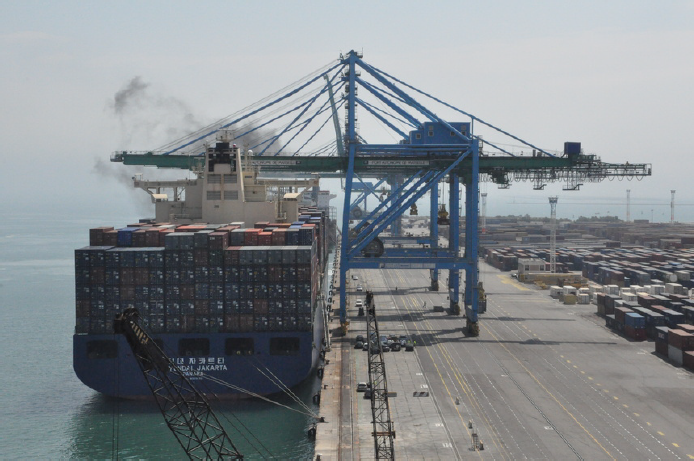
\includegraphics[width=.7\linewidth]{images/fig_00}
}%figues de la page de garde


\def\xxpied{%
Cycle 04 -- Modélisation mécanique -- PFD\\% afin de valider leurs performances.\\
Chapitre 4 -- \xxactivite%
}

\setcounter{secnumdepth}{5}
%---------------------------------------------------------------------------

\usepackage{pgfplots}
\begin{document}
\def\pathfig{images}
%\chapterimage{png/Fond_Cin}
\pagestyle{empty}


%%%%%%%% PAGE DE GARDE COURS
\ifcours
% ==== BANDEAU DES TITRES ==== 
\begin{tikzpicture}[remember picture,overlay]
\node at (current page.north west)
{\begin{tikzpicture}[remember picture,overlay]
\node[anchor=north west,inner sep=0pt] at (0,0) {\includegraphics[width=\paperwidth]{\thechapterimage}};
\draw[anchor=west] (-2cm,-8cm) node [line width=2pt,rounded corners=15pt,draw=ocre,fill=white,fill opacity=0.6,inner sep=40pt]{\strut\makebox[22cm]{}};
\draw[anchor=west] (1cm,-8cm) node {\huge\sffamily\bfseries\color{black} %
\begin{minipage}{1cm}
\rotatebox{90}{\LARGE\sffamily\textsc{\color{ocre}\textbf{\xxnumpartie}}}
\end{minipage} \hfill
\begin{minipage}[c]{14cm}
\begin{titrepartie}
\begin{flushright}
\renewcommand{\baselinestretch}{1.1} 
\Large\sffamily\textsc{\textbf{\xxpartie}}
\renewcommand{\baselinestretch}{1} 
\end{flushright}
\end{titrepartie}
\end{minipage} \hfill
\begin{minipage}[c]{3.5cm}
{\large\sffamily\textsc{\textbf{\color{ocre} \discipline}}}
\end{minipage} 
 };
\end{tikzpicture}};
\end{tikzpicture}
% ==== FIN BANDEAU DES TITRES ==== 


% ==== ONGLET 
\begin{tikzpicture}[overlay]
\node[shape=rectangle, 
      rounded corners = .25 cm,
	  draw= ocre,
	  line width=2pt, 
	  fill = ocre!10,
	  minimum width  = 2.5cm,
	  minimum height = 3cm,] at (18.3cm,0) {};
\node at (17.7cm,0) {\rotatebox{90}{\textbf{\Large\color{ocre}{\classe}}}};
%{};
\end{tikzpicture}
% ==== FIN ONGLET 


\vspace{3.5cm}

\begin{tikzpicture}[remember picture,overlay]
\draw[anchor=west] (-2cm,-6cm) node {\huge\sffamily\bfseries\color{black} %
\begin{minipage}{2cm}
\begin{center}
\LARGE\sffamily\textsc{\color{ocre}\textbf{\xxactivite}}
\end{center}
\end{minipage} \hfill
\begin{minipage}[c]{15cm}
\begin{titrechapitre}
\renewcommand{\baselinestretch}{1.1} 
\Large\sffamily\textsc{\textbf{\xxnumchapitre}}

\Large\sffamily\textsc{\textbf{\xxchapitre}}
\vspace{.5cm}

\renewcommand{\baselinestretch}{1} 
\normalsize\normalfont
\xxcompetences
\end{titrechapitre}
\end{minipage}  };
\end{tikzpicture}
\vfill

\begin{flushright}
\begin{minipage}[c]{.3\linewidth}
\begin{center}
\xxfigures
\end{center}
\end{minipage}\hfill
\begin{minipage}[c]{.6\linewidth}
\startcontents
%\printcontents{}{1}{}
\printcontents{}{1}{}
\end{minipage}
\end{flushright}

\begin{tikzpicture}[remember picture,overlay]
\draw[anchor=west] (4.5cm,-.7cm) node {
\begin{minipage}[c]{.2\linewidth}
\begin{flushright}

\includegraphics[width=2cm]{logoCC}
\end{flushright}
\end{minipage}
\begin{minipage}[c]{.2\linewidth}
\textsl{\xxauteur} \\
\textsl{\classe}
\end{minipage}
 };
\end{tikzpicture}

\newpage
\pagestyle{fancy}

%\newpage
%\pagestyle{fancy}

\else
\fi
%% FIN PAGE DE GARDE DES COURS

%%%%%%%% PAGE DE GARDE TD
\iftd
%\begin{tikzpicture}[remember picture,overlay]
%\node at (current page.north west)
%{\begin{tikzpicture}[remember picture,overlay]
%\draw[anchor=west] (-2cm,-3.25cm) node [line width=2pt,rounded corners=15pt,draw=ocre,fill=white,fill opacity=0.6,inner sep=40pt]{\strut\makebox[22cm]{}};
%\draw[anchor=west] (1cm,-3.25cm) node {\huge\sffamily\bfseries\color{black} %
%\begin{minipage}{1cm}
%\rotatebox{90}{\LARGE\sffamily\textsc{\color{ocre}\textbf{\xxnumpartie}}}
%\end{minipage} \hfill
%\begin{minipage}[c]{13.5cm}
%\begin{titrepartie}
%\begin{flushright}
%\renewcommand{\baselinestretch}{1.1} 
%\Large\sffamily\textsc{\textbf{\xxpartie}}
%\renewcommand{\baselinestretch}{1} 
%\end{flushright}
%\end{titrepartie}
%\end{minipage} \hfill
%\begin{minipage}[c]{3.5cm}
%{\large\sffamily\textsc{\textbf{\color{ocre} \discipline}}}
%\end{minipage} 
% };
%\end{tikzpicture}};
%\end{tikzpicture}

%%%%%%%%%% PAGE DE GARDE TD %%%%%%%%%%%%%%%
%\begin{tikzpicture}[overlay]
%\node[shape=rectangle, 
%      rounded corners = .25 cm,
%	  draw= ocre,
%	  line width=2pt, 
%	  fill = ocre!10,
%	  minimum width  = 2.5cm,
%	  minimum height = 2.5cm,] at (18.5cm,0) {};
%\node at (17.7cm,0) {\rotatebox{90}{\textbf{\Large\color{ocre}{\classe}}}};
%%{};
%\end{tikzpicture}

% PARTIE ET CHAPITRE
%\begin{tikzpicture}[remember picture,overlay]
%\draw[anchor=west] (-1cm,-2.1cm) node {\large\sffamily\bfseries\color{black} %
%\begin{minipage}[c]{15cm}
%\begin{flushleft}
%\xxnumchapitre \\
%\xxchapitre
%\end{flushleft}
%\end{minipage}  };
%\end{tikzpicture}

% BANDEAU EXO
\iflivret % SI LIVRET
\begin{tikzpicture}[remember picture,overlay]
\draw[anchor=west] (-2cm,-3.3cm) node {\huge\sffamily\bfseries\color{black} %
\begin{minipage}{5cm}
\begin{center}
\LARGE\sffamily\color{ocre}\textbf{\textsc{\xxactivite}}

\begin{center}
\xxfigures
\end{center}

\end{center}
\end{minipage} \hfill
\begin{minipage}[c]{12cm}
\begin{titrechapitre}
\renewcommand{\baselinestretch}{1.1} 
\large\sffamily\textbf{\textsc{\xxtitreexo}}

\small\sffamily{\textbf{\textit{\color{black!70}\xxsourceexo}}}
\vspace{.5cm}

\renewcommand{\baselinestretch}{1} 
\normalsize\normalfont
\xxcompetences
\end{titrechapitre}
\end{minipage}};
\end{tikzpicture}
\else % ELSE NOT LIVRET
\begin{tikzpicture}[remember picture,overlay]
\draw[anchor=west] (-2cm,-4.5cm) node {\huge\sffamily\bfseries\color{black} %
\begin{minipage}{5cm}
\begin{center}
\LARGE\sffamily\color{ocre}\textbf{\textsc{\xxactivite}}

\begin{center}
\xxfigures
\end{center}

\end{center}
\end{minipage} \hfill
\begin{minipage}[c]{12cm}
\begin{titrechapitre}
\renewcommand{\baselinestretch}{1.1} 
\large\sffamily\textbf{\textsc{\xxtitreexo}}

\small\sffamily{\textbf{\textit{\color{black!70}\xxsourceexo}}}
\vspace{.5cm}

\renewcommand{\baselinestretch}{1} 
\normalsize\normalfont
\xxcompetences
\end{titrechapitre}
\end{minipage}};
\end{tikzpicture}

\fi

\else   % FIN IF TD
\fi


%%%%%%%% PAGE DE GARDE FICHE
\iffiche
\begin{tikzpicture}[remember picture,overlay]
\node at (current page.north west)
{\begin{tikzpicture}[remember picture,overlay]
\draw[anchor=west] (-2cm,-2.25cm) node [line width=2pt,rounded corners=15pt,draw=ocre,fill=white,fill opacity=0.6,inner sep=40pt]{\strut\makebox[22cm]{}};
\draw[anchor=west] (1cm,-2.25cm) node {\huge\sffamily\bfseries\color{black} %
\begin{minipage}{1cm}
\rotatebox{90}{\LARGE\sffamily\textsc{\color{ocre}\textbf{\xxnumpartie}}}
\end{minipage} \hfill
\begin{minipage}[c]{14cm}
\begin{titrepartie}
\begin{flushright}
\renewcommand{\baselinestretch}{1.1} 
\large\sffamily\textsc{\textbf{\xxpartie} \\} 

\vspace{.2cm}

\normalsize\sffamily\textsc{\textbf{\xxnumchapitre -- \xxchapitre}}
\renewcommand{\baselinestretch}{1} 
\end{flushright}
\end{titrepartie}
\end{minipage} \hfill
\begin{minipage}[c]{3.5cm}
{\large\sffamily\textsc{\textbf{\color{ocre} \discipline}}}
\end{minipage} 
 };
\end{tikzpicture}};
\end{tikzpicture}

\iflivret
\begin{tikzpicture}[overlay]
\node[shape=rectangle, 
      rounded corners = .25 cm,
	  draw= ocre,
	  line width=2pt, 
	  fill = ocre!10,
	  minimum width  = 2.5cm,
	  minimum height = 2.5cm,] at (18.5cm,.5cm) {};
\node at (17.9cm,.5cm) {\rotatebox{90}{\textsf{\textbf{\large\color{ocre}{\classe}}}}};
%{};
\end{tikzpicture}
\else
\begin{tikzpicture}[overlay]
\node[shape=rectangle, 
      rounded corners = .25 cm,
	  draw= ocre,
	  line width=2pt, 
	  fill = ocre!10,
	  minimum width  = 2.5cm,
%	  minimum height = 2.5cm,] at (18.5cm,1.1cm) {};
	  minimum height = 2.5cm,] at (18.6cm,0.5cm) {};
\node at (18cm,0.5cm) {\rotatebox{90}{\textsf{\textbf{\large\color{ocre}{\classe}}}}};
%{};
\end{tikzpicture}

\fi

\else
\fi



\vspace{5cm}
\pagestyle{fancy}
\thispagestyle{plain}

\def\columnseprulecolor{\color{ocre}}
\setlength{\columnseprule}{0.4pt} 

\def\pathfig{images}

\ifprof
\else
\begin{multicols}{2}
\fi

\subsection*{Modélisation dynamique du comportement de la charge}

\begin{obj}
Déterminer les équations du mouvement du conteneur de façon à en obtenir un modèle simple pour
la synthèse de la commande.
\end{obj}

\ifprof
\else
En vue d’élaborer une commande automatisée du déchargement des conteneurs, une bonne compréhension de
la dynamique du système est nécessaire. Cette partie vise à établir les équations du mouvement du conteneur.
%Seul le vérin 3 est libéré. 
La charge peut alors balancer selon le modèle présenté ci-après. Dans cette étude, la vitesse de vent nulle. On fait l'hypothèse que le conteneur est suspendu à un seul câble indéformable, en liaison pivot à ses extrémités. Les liaisons entre les solides 0, 1, 2 et 3 sont supposées parfaites.
Le portique support du chariot est noté 0, le chariot 1, le câble 2 et l’ensemble \{spreader + conteneur\} 3.

\paragraph*{Paramétrage}
\begin{itemize}
\item Le repère $\mathcal{R}_0=\repere{O_0}{x_0}{y_0}{z_0}$ est lié au portique fixe ; il est supposé
galiléen avec $\vect{z_0}$ l’axe vertical ascendant.
\item La position du chariot telle que $\vect{OE} = y_{ch}(t) \vect{y_0}$ est notée $y_{ch}(t)$ ;
l’angle $\angl{z_0}{z_2}$ d’inclinaison du câble $\theta(t)$ et l’angle $\angl{z_2}{z_3}$ d’inclinaison
du conteneur par rapport au câble  $\beta(t)$.
\end{itemize}


\paragraph*{Données}
\begin{itemize}
\item $\mathcal{R}_1=\repere{E}{x_0}{y_0}{z_0}$  repère lié au chariot de levage 1.
\item $\mathcal{R}_2=\repere{E}{x_0}{y_2}{z_2}$  repère lié au câble 2; $\ell_2 = \SI{50}{m}$ la longueur $EF$
du câble ; la masse est négligée.
\item $\mathcal{R}_3=\repere{F}{x_0}{y_3}{z_3}$  repère lié à l’ensemble \{spreader + conteneur\};
$m_3 = \SI{50}{tonnes}$ la masse du solide 3 ; $G_3$ le centre de gravité du
solide 3, tel que $\vect{G_3F}=h_3\vect{z_3}$ où $h_3 = \SI{2,5}{m}$; la matrice d’inertie du solide 3 s’écrit
$\inertie{3}{G_3}=\matinertie{A_3}{B_3}{C_3}{0}{0}{0}{\left(\vect{x_0},\vect{y_3},\vect{z_3} \right)}$ où $\left| \begin{array}{l} A_3 = \SI{52e3}{kg.m^2} \\ B_3 = \SI{600e3}{kg.m^2} \\ C_3 = \SI{600e3}{kg.m^2} \end{array}\right.$. 
\item la motorisation $M_D$ du mouvement de direction exerce, par l’intermédiaire de câbles, des actions mécaniques sur (1) qui se réduisent
à un glisseur de la forme $\vectf{M_D}{1} =F \vect{y_0}$ ;
\item l’action mécanique du câble sur le spreader est notée $\vectf{2}{3} =F_{23} \vect{z_2}$.
\end{itemize}



\begin{center}
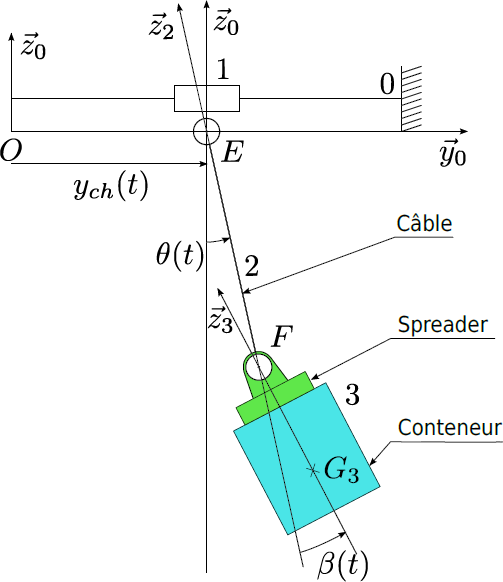
\includegraphics[width=.8\linewidth]{images/fig_01}
\end{center}

\fi

\subparagraph{}
\textit{Après avoir réalisé le graphe de structure, déterminer le nombre de degrés de liberté et le nombre d’actionneurs du modèle proposé figure précédente. En
déduire le nombre de degrés de liberté non motorisés. Expliquer pourquoi il est difficile de poser le conteneur
sur un camion avec précision ?}
\ifprof
\begin{corrige} ~\\

\begin{center}
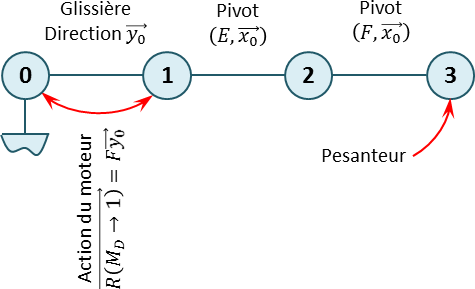
\includegraphics[width=.5\linewidth]{images/cor_01}
\hfill
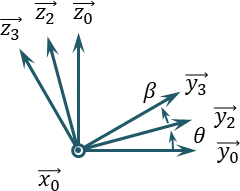
\includegraphics[width=.3\linewidth]{images/cor_02}
\end{center}

Le système a trois mobilités : 
\begin{itemize}
\item la translation de la liaison glissière de longueur $y_{ch}(t)$ (degré de liberté motorisé);
\item la rotation du câble d'angle $\theta(t)$ (degré de liberté non motorisé);
\item la rotation du conteneur d'angle $\beta(t)$ (degré de liberté non motorisé). 
\end{itemize}

Les deux liaisons pivot n'étant pas freinées ou motorisées, lorsque le chariot se positionne au-dessus du camion le conteneur va se balancer, ce qui rend difficile la dépose du conteneur. 

\end{corrige}
\else
\fi


\subparagraph{}
\textit{Déterminer littéralement, au point $G_3$, la vitesse $\vectv{G_3}{3}{0}$ puis le torseur dynamique $\torseurdyn{3}{0}$ de l’ensemble \{conteneur + spreader\} (3) dans son mouvement par rapport au repère galiléen $\mathcal{R}_0$.}
\ifprof
\begin{corrige}
$\vectv{G_3}{3}{0}=   \left[\dfrac{\dd \vect{OG_3}}{\dd t}\right]_{\rep{0}}=   \left[\dfrac{\dd }{\dd t}\left(
\vect{OE}+\vect{EF}+\vect{FG_3} \right)\right]_{\rep{0}}$ 
$=   \left[\dfrac{\dd }{\dd t}\left(
y_{ch}(t) \vect{y_0}-\ell_2\vect{z_2}-h_3\vect{z_3} \right)\right]_{\rep{0}}$. 

On a : 
\begin{itemize}
\item $ \left[\dfrac{\dd \vect{z_2}}{\dd t}\right]_{\rep{0}}=\left[\dfrac{\dd \vect{z_2}}{\dd t}\right]_{\rep{2}}+\vecto{2}{0} \wedge \vect{z_2}=\dot{\theta} \vect{x_2}\wedge \vect{z_2}=-\dot{\theta} \vect{y_2}$;
\item $ \left[\dfrac{\dd \vect{z_3}}{\dd t}\right]_{\rep{0}}=\left[\dfrac{\dd \vect{z_3}}{\dd t}\right]_{\rep{3}}+\vecto{3}{0} \wedge \vect{z_3}=\left(\dot{\theta}+\dot{\beta}\right) \vect{x_2}\wedge \vect{z_3}=-\left(\dot{\theta}+\dot{\beta}\right) \vect{y_3}$;
\item $ \left[\dfrac{\dd \vect{y_2}}{\dd t}\right]_{\rep{0}}=\dot{\theta} \vect{z_2}$;
\item $ \left[\dfrac{\dd \vect{y_3}}{\dd t}\right]_{\rep{0}}=\left(\dot{\theta}+\dot{\beta}\right) \vect{z_3}$.
\end{itemize}

$\vectv{G_3}{3}{0}=   
\dot{y}_{ch}(t) \vect{y_0}+\ell_2\dot{\theta} \vect{y_2}+h_3\left(\dot{\theta}+\dot{\beta}\right) \vect{y_3}$.

$\vectg{G_3}{3}{0}=   
\ddot{y}_{ch}(t) \vect{y_0}+\ell_2\ddot{\theta} \vect{y_2}+h_3\left(\ddot{\theta}+\ddot{\beta}\right) \vect{y_3}
+   
\ell_2\dot{\theta}^2 \vect{z_2}  +h_3\left(\dot{\theta}+\dot{\beta}\right)^2\vect{z_3} $.

Par ailleurs, $G_3$ étant le centre d'inertie, de 3, on a $\vectmd{G_3}{3}{0}=\left[\dfrac{\dd \vectmc{G_3}{3}{0}}{\dd t}\right]_{\rep{0}}=\left[\dfrac{\dd A_3 \left(\dot{\theta}+\dot{\beta} \right)\vect{x_0}}{\dd t}\right]_{\rep{0}}=A_3 \left(\ddot{\theta}+\ddot{\beta} \right)\vect{x_0}$.

On a donc, $\torseurdyn{3}{0}=\torseurl{M_3\left(\ddot{y}_{ch}(t) \vect{y_0}+\ell_2\ddot{\theta} \vect{y_2}+h_3\left(\ddot{\theta}+\ddot{\beta}\right) \vect{y_3}
+   
\ell_2\dot{\theta}^2 \vect{z_2}  +h_3\left(\dot{\theta}+\dot{\beta}\right)^2\vect{z_3}\right)}{A_3 \left(\ddot{\theta}+\ddot{\beta} \right)\vect{x_0}}{G_3}$
\end{corrige}
\else
\fi


\subparagraph{}
\textit{En précisant l’isolement et le bilan des actions mécaniques extérieures, déterminer l’équation différentielle
de résultante reliant les paramètres $\theta(t)$, $\beta(t)$%$\beta(t)$
 et $y_{ch}(t)$, sans inconnue de liaison et sans l'action du moteur.}
\ifprof
\begin{corrige}

D'une part, on peut se dire qu'on va utiliser le résultat de la question précédente. D'autre part, le sujet demande une équation de résultante sans aucune action mécanique. Si on isole le solide 3, il va donc falloir projeter sur une direction ne faisant pas intervenir d'action mécanique. Les données précisent que l'action du câble est suivant $\vect{z_2}$, on peut donc suggérer de réaliser le thorème de la résultante dynamique appliqué au solide 3 en projection sur $\vect{y_2}$. 

Le bilan des actions mécaniques est donc le suivant : 
\begin{itemize}
\item action de la pesanteur sur 3;
\item action de 2 sur 3.
\end{itemize}

On a donc :
$-M_3 g \vect{z_0}\cdot \vect{y_2} = 
\left( M_3\left(\ddot{y}_{ch}(t) \vect{y_0}+\ell_2\ddot{\theta} \vect{y_2}+h_3\left(\ddot{\theta}+\ddot{\beta}\right) \vect{y_3}
+   
\ell_2\dot{\theta}^2 \vect{z_2}  +h_3\left(\dot{\theta}+\dot{\beta}\right)^2\vect{z_3}\right)\right) \cdot \vect{y_2}$

$ \Leftrightarrow -M_3 g \sin \theta  = 
 M_3\left(\ddot{y}_{ch}(t) \cos \theta +\ell_2\ddot{\theta} +h_3\left(\ddot{\theta}+\ddot{\beta}\right)\cos \beta 
-h_3\left(\dot{\theta}+\dot{\beta}\right)^2\sin\beta \right)$


\vspace{.6cm}
Résolution faisant intervenir $F$ -- Non demandé.

L'équation de résultante étant demandée, on peut aussi isoler une pièce (ou un ensemble de pièces) en translation rectiligne. On isole donc \textbf{(1+2+3)} et on réalise un théorème de la résultante dynamique en projection sur $\vect{y_0}$. 

Bilan des actions mécaniques : 
\begin{itemize}
\item action de la pesanteur sur 3 (la résultante n'a pas de composante sur $\vect{y_0}$);
\item action de la pesanteur sur 1 (négligée) (la résultante n'a pas de composante sur $\vect{y_0}$);
\item action de 0 sur 3 (glissière) (la résultante n'a pas de composante sur $\vect{y_0}$);
\item action du moteur sur 1.
\end{itemize}

On applique le TRD sur $\vect{y_0}$ :
$F = \vectrd{1+2+3}{0}\cdot \vect{y_0}= \underbrace{\vectrd{1}{0} \cdot  \vect{y_0}}_{=0 \text{(masse négligée)}}+ \underbrace{\vectrd{2}{0}\cdot  \vect{y_0}}_{=0 \text{(masse négligée)}} + \vectrd{3}{0}\cdot \vect{y_0}$

 $ \Rightarrow F = \left( M_3\left(\ddot{y}_{ch}(t) \vect{y_0}+\ell_2\ddot{\theta} \vect{y_2}+h_3\left(\ddot{\theta}+\ddot{\beta}\right) \vect{y_3}
+   
\ell_2\dot{\theta}^2 \vect{z_2}  +h_3\left(\dot{\theta}+\dot{\beta}\right)^2\vect{z_3}\right)\right) \cdot \vect{y_0}$

 $ \Leftrightarrow F =  M_3\left(\ddot{y}_{ch}(t) +\ell_2\ddot{\theta} \cos \theta +h_3\left(\ddot{\theta}+\ddot{\beta}\right) \cos \left( \beta+\theta\right)
-
\ell_2\dot{\theta}^2 \sin \theta   -h_3\left(\dot{\theta}+\dot{\beta}\right)^2  \sin \left( \beta+\theta\right)\right) $
\end{corrige}
\else
\fi


\subparagraph{}
\textit{En précisant l’isolement et le bilan des actions mécaniques extérieures, déterminer les équations différentielles
reliant les paramètres $\theta(t)$, $\beta(t)$  et $y_{ch}(t)$ et sans inconnue de liaison. La méthode sera clairement séparée des calculs.}
\ifprof
\begin{corrige}
Le TRD appliqué à 3 en projection suivant $\vect{z_2}$ se traduit par : 

$F-M_3 g \vect{z_0}\cdot \vect{z_2} = 
\left( M_3\left(\ddot{y}_{ch}(t) \vect{y_0}+\ell_2\ddot{\theta} \vect{y_2}+h_3\left(\ddot{\theta}+\ddot{\beta}\right) \vect{y_3}
+   
\ell_2\dot{\theta}^2 \vect{z_2}  +h_3\left(\dot{\theta}+\dot{\beta}\right)^2\vect{z_3}\right)\right) \cdot \vect{z_2}$

$\Leftrightarrow F-M_3 g \cos \theta  = 
 M_3\left(- \ddot{y}_{ch}(t) \sin \theta +h_3\left(\ddot{\theta}+\ddot{\beta}\right) \sin\beta
+   
\ell_2\dot{\theta}^2   +h_3\left(\dot{\theta}+\dot{\beta}\right)^2\cos \beta \right) $.



Le TMD appliqué à 3 au point $F$ en projection suivant $\vect{x_0}$ se traduit par : 

$\vect{FG_3}\wedge \left(-M_3g \vect{z_0} \right) \cdot \vect{x_0} =\left(\vectmd{G_3}{3}{0}+\vect{FG_3}\wedge \vectrd{3}{0}\right)\cdot \vect{x_0}$

$\Leftrightarrow -h_3 \vect{z_3} \wedge \left(-M_3g \vect{z_0} \right) \cdot \vect{x_0} =A_3 \left(\ddot{\theta}+\ddot{\beta} \right)$

$\Leftrightarrow - M_3gh_3 \sin\left( \beta + \theta\right) =A_3 \left(\ddot{\theta}+\ddot{\beta} \right)$.
\end{corrige}
\else
\fi


\subparagraph{}
\textit{En supposant que $\theta$, $\beta$, $\dot{\theta}$ et $\dot{\beta}$ sont petits, linéariser les équations précédentes.  }
\ifprof
\begin{corrige}
\begin{itemize}
\item On a 
$ -M_3 g \sin \theta  = 
 M_3\left(\ddot{y}_{ch}(t) \cos \theta +\ell_2\ddot{\theta} +h_3\left(\ddot{\theta}+\ddot{\beta}\right)\cos \beta 
-h_3\left(\dot{\theta}+\dot{\beta}\right)^2\sin\beta \right)$. En linéarisant, on obtient 
$ -M_3 g \theta  = 
 M_3\left(\ddot{y}_{ch}(t) +\ell_2\ddot{\theta} +h_3\left(\ddot{\theta}+\ddot{\beta}\right) 
-h_3\left(\dot{\theta}+\dot{\beta}\right)^2\beta \right)$. En considérant que $\dot{\theta}$ et $\dot{\beta}$ sont petits, on a : 
$ -M_3 g \theta  = 
 M_3\left(\ddot{y}_{ch}(t) +\ell_2\ddot{\theta} +h_3\left(\ddot{\theta}+\ddot{\beta}\right)  \right)$.
\item  On a : $F-M_3 g \cos \theta  = 
 M_3\left(- \ddot{y}_{ch}(t) \sin \theta +h_3\left(\ddot{\theta}+\ddot{\beta}\right) \sin\beta
+   
\ell_2\dot{\theta}^2   +h_3\left(\dot{\theta}+\dot{\beta}\right)^2\cos \beta \right) $. En linéarisant, on obtient :
$F-M_3 g  = 
 M_3\left(- \ddot{y}_{ch}(t) \theta +h_3\left(\ddot{\theta}+\ddot{\beta}\right) \beta
+   
\ell_2\dot{\theta}^2   +h_3\left(\dot{\theta}+\dot{\beta}\right)^2 \right) $
En considérant que $\dot{\theta}$ et $\dot{\beta}$ sont petits, on a : 
$F-M_3 g  = 
 M_3\left(- \ddot{y}_{ch}(t) \theta +h_3\left(\ddot{\theta}+\ddot{\beta}\right) \beta
 \right) $.
 \item On a : $ M_3gh_3 \sin\left( \beta + \theta\right) =A_3 \left(\ddot{\theta}+\ddot{\beta} \right)$ En linéarisant, on obtient  $M_3gh_3 \left( \beta + \theta\right) =A_3 \left(\ddot{\theta}+\ddot{\beta} \right)$.
 \end{itemize}

\end{corrige}
\else
\fi


Les courbes temporelles ont été obtenues par simulation, à partir des équations précédentes, pour un
échelon en $y_{ch}(t)$ de $\SI{10}{m}$. 

\ifprof
\begin{multicols}{2}
\begin{center}
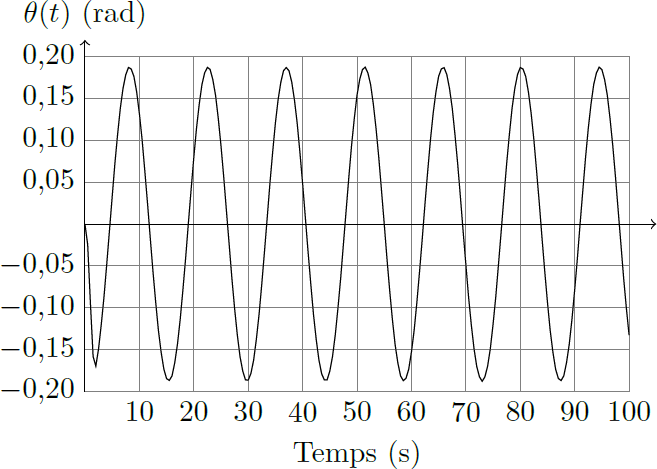
\includegraphics[width=.8\linewidth]{images/fig_02}
\end{center}

\begin{center}
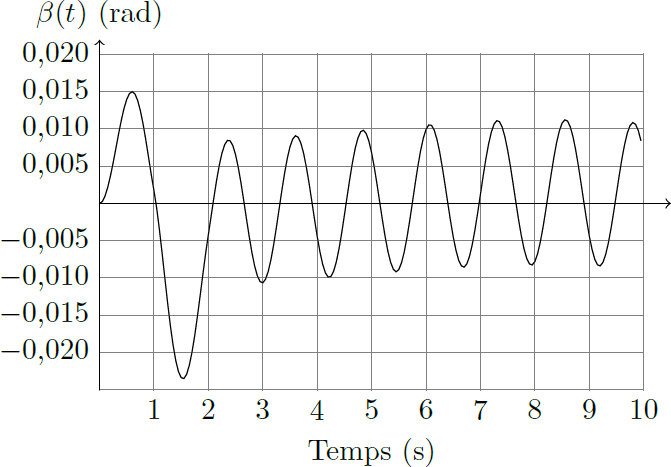
\includegraphics[width=.8\linewidth]{images/fig_03}
\end{center}
\end{multicols}
\else
\fi



\subparagraph{}
\textit{Proposer une simplification de la modélisation précédente.   }
\ifprof
\begin{corrige}
L'amplitude des oscillations de $\beta$ est 10 fois inférieure aux oscillations de $\theta$. En conséquences, on pourrait poser $\beta=0$ et :

\begin{itemize}
\item $ - g \theta  = \ddot{y}_{ch}(t) +\ell_2\ddot{\theta} +h_3\ddot{\theta} $;
\item  $F-M_3 g  = - M_3 \ddot{y}_{ch}(t) \theta  $;
 \item  $M_3gh_3 \theta =A_3 \ddot{\theta} $.
 \end{itemize}
 
\end{corrige}
\else
\fi



%\begin{itemize}
%\item $\mathcal{R}_0=\repere{O_0}{x_0}{y_0}{z_0}$ est un repère supposé galiléen, où $\vect{x_0}$ est dirigé suivant la vitesse de la moto et $\vect{y_0}$ suivant la verticale ascendante;
%\item $\mathcal{R}_1=\repere{G_1}{x_1}{y_1}{z_1}$ est un repère lié à l'ensemble considéré indéformable \{cadre + bras arrière + fourche avant + pilote\}. On note $\theta_1=\angl{x_0}{x_1}$;
%\item $\mathcal{R}_2=\repere{O_2}{x_2}{y_2}{z_2}$ est un repère lié à la roue avant (2), de rayon $R$ et de centre $O_2$ tel que $\vect{z_2}=\vect{z_0}$. On note $\theta_2=\angl{x_0}{x_2}$;
%\item $\mathcal{R}_3=\repere{O_3}{x_3}{y_3}{z_3}$ est un repère lié à la roue arrière (3), de rayon $R$ et de centre $O_3$ tel que $\vect{z_3}=\vect{z_0}$. On note $\theta_3=\angl{x_0}{x_3}$. Les contacts entre les roues \textbf{(2)} et \textbf{(3)} et le sol \textbf{(0)} sont modélisés par des liaisons ponctuelles en $H_2$ et $H_3$.
%\end{itemize}
%
%On note :
%\begin{itemize}
%\item $\vect{OO_3} = \lambda \vect{x_0}+R\vect{y_0}$;
%\item $\vect{O_3O_2} = L_1\vect{x_1}$;
%\item $\vect{O_3G_1} = a_1\vect{x_1}+b_1\vect{y_1}$;
%\item $\vect{H_3O_3} = R \vect{y_0}$;
%\item $\vect{H_2O_2} = R \vect{y_0}$;
%\item $G_2 = O_2$ et $G_3 = O_3$.
%\end{itemize}
%
%On note $G_i$ le centre d'inertie, $m_i$ la masse et $C_i$ le moment d'inertie par rapport à l'axe   de la pièce \textbf{(i)}. 
%
%\subsection*{Étude dynamique}
%La transmission exerce sur la roue arrière un couple moteur $\vect{C_m}=C_m\vect{z_0}$. 
%On suppose que l’adhérence roue/sol est suffisante pour assurer le roulement sans glissement de la roue \textbf{(3)} au contact en $H$ avec le sol.
%La situation initiale est définie au moment où la roue avant quitte le contact avec le sol, avec   $\dot{\theta_1}=0$ (après $\neq 0$).
%
%
%\subparagraph{}
%\textit{Construire le graphe de structure de la moto dans la phase de wheeling.
%Préciser le degré de mobilité de l'ensemble, compte tenu de l'hypothèse de roulement sans glissement en $H_3$.}
%\ifprof
%\begin{corrige}
%\end{corrige}
%\else
%\fi
%
%\subparagraph{}
%\textit{En se limitant à l'application des théorèmes généraux de la dynamique, définir quelles équations permettent de déterminer le mouvement de l'ensemble, en précisant:
%\begin{itemize}
%\item élément(s) isolé(s) ;
%\item théorème appliqué, en précisant quelle projection et quel point de réduction éventuel sont retenus. 
%\end{itemize}
%}
%
%\ifprof
%\begin{corrige}
%\end{corrige}
%\else
%\fi
%
%
%\subparagraph{}
%\textit{Mettre en place les équations précédentes.
%Conclure sur la possibilité d'intégration de ces équations. }
%\ifprof
%\begin{corrige}
%\end{corrige}
%\else
%\fi
%

\ifprof
\else
\end{multicols}x
\fi


%\begin{center}
%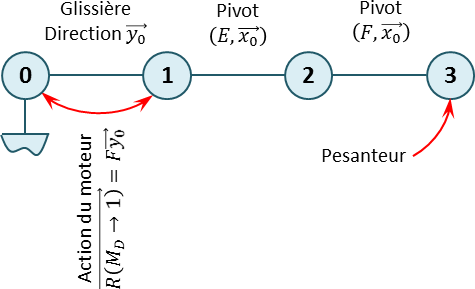
\includegraphics[width=\linewidth]{images/cor_01}
%\end{center}
%
%\begin{center}
%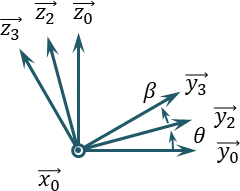
\includegraphics[width=\linewidth]{images/cor_02}
%\end{center}
%
%\begin{center}
%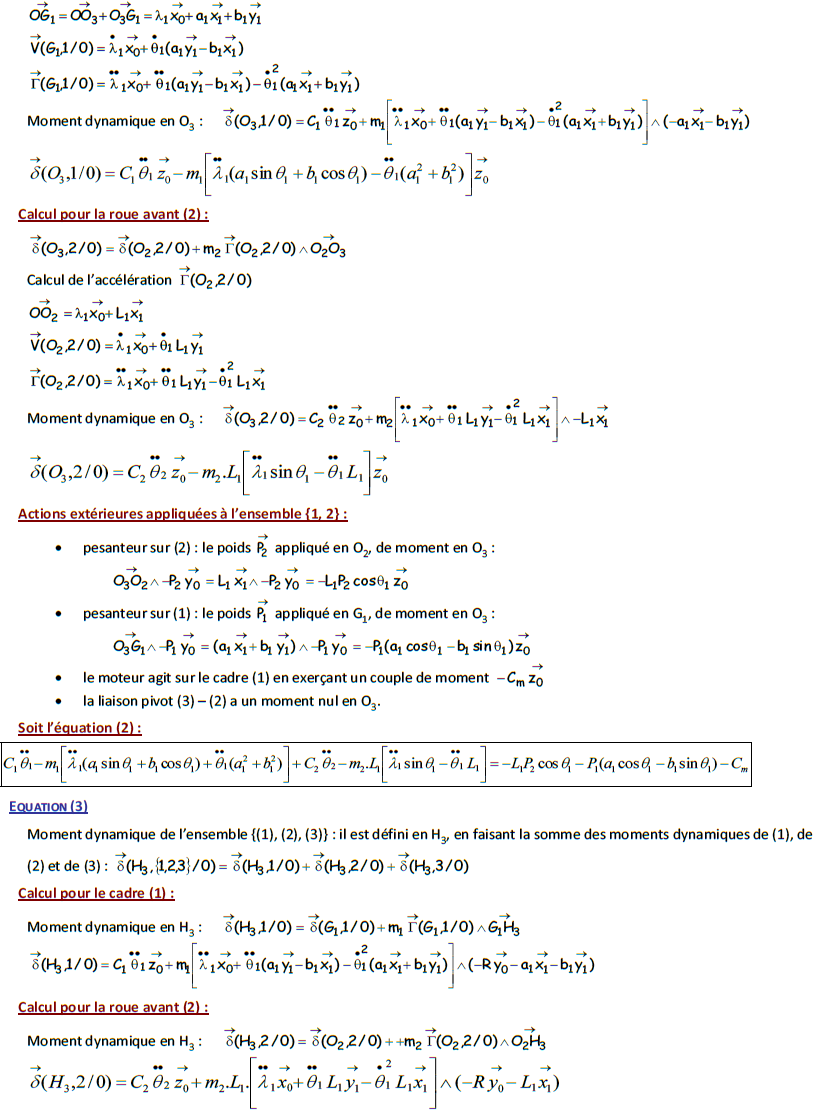
\includegraphics[width=\linewidth]{images/cor_03}
%\end{center}
%
%\begin{center}
%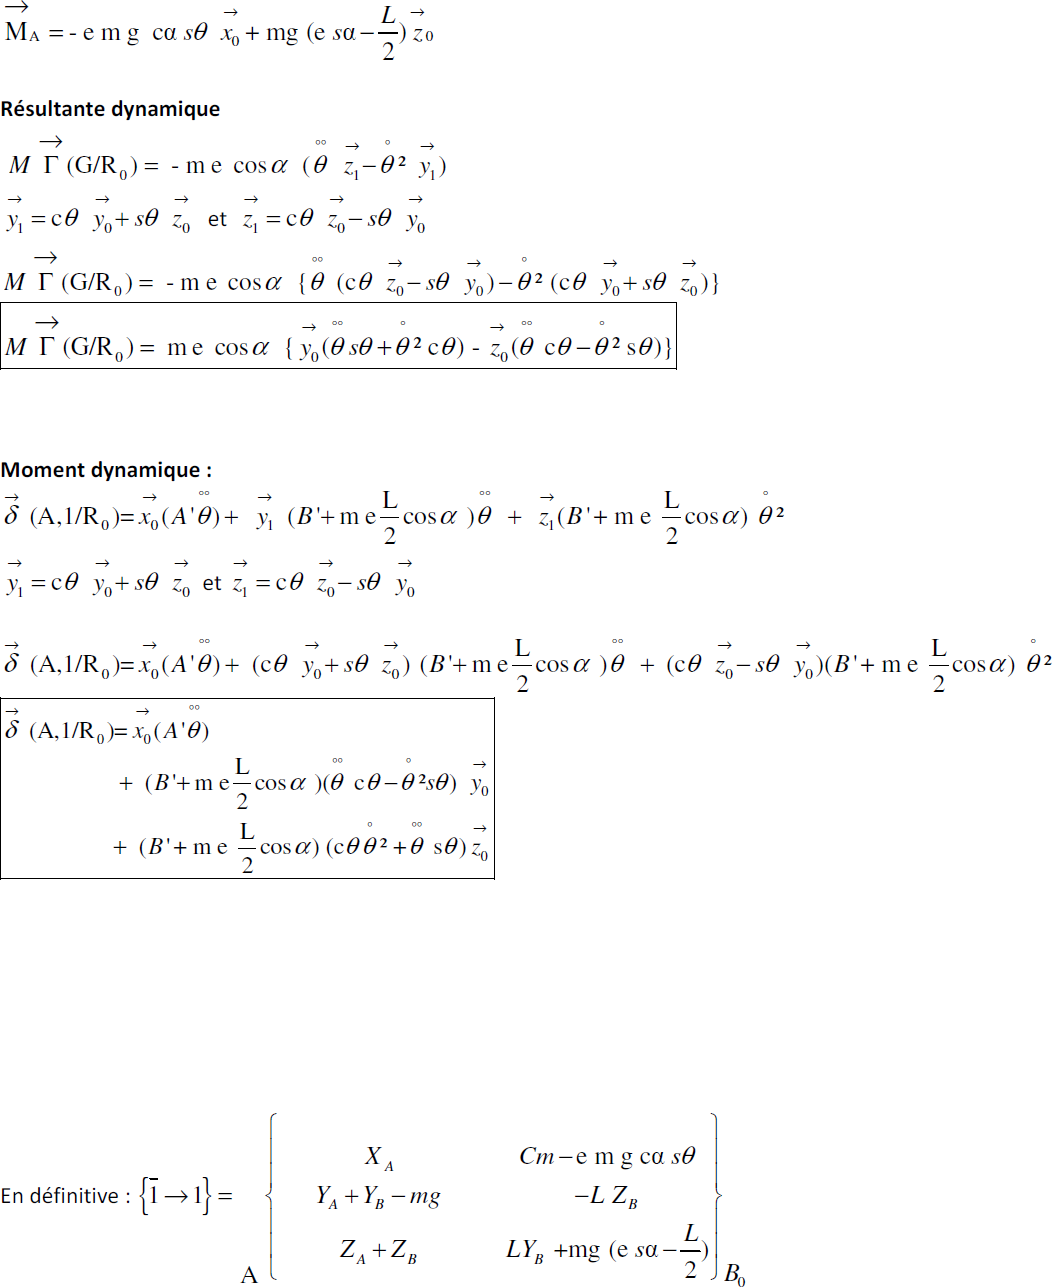
\includegraphics[width=\linewidth]{images/cor_04}
%\end{center}

%\begin{center}
%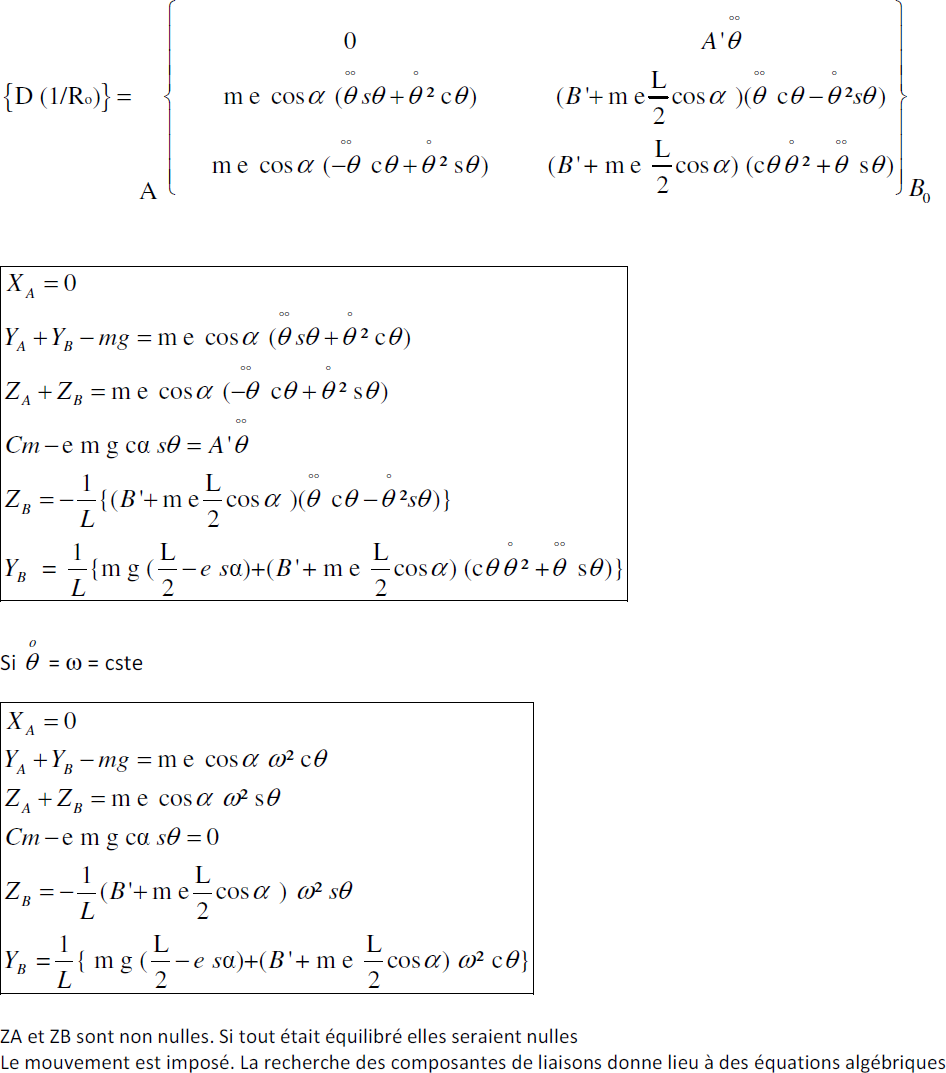
\includegraphics[width=\linewidth]{images/cor_05}
%\end{center}


\end{document}
\begin{center}
\includegraphics[width=\linewidth]{images/}
\end{center}

\subparagraph{}
\textit{}
\ifprof
\begin{corrige}
\end{corrige}
\else
\fi
